\ylDisplay{Toru} % Ülesande nimi
{Tundmatu autor} % Autor
{lahtine} % Voor
{2007} % Aasta
{G 2} % Ülesande nr.
{2} % Raskustase
{
% Teema: Staatika
\ifStatement
Kaks inimest kannavad toru massiga $m = \SI{80}{kg}$ ja pikkusega $l = \SI{5}{m}$. Esimene inimene hoiab toru kaugusel $a = \SI{1}{m}$ toru otsast, teine aga hoiab toru teist otsa. Leida jõud, mida toru avaldab igale inimesele.
\fi


\ifHint
Kehtib Newtoni II seadus ning jõumomentide tasakaal (näiteks ühe toru otspunkti suhtes).
\fi


\ifSolution
Newtoni kolmanda seaduse kohaselt on toru toereaktsioonid $N_1$ ja $N_2$ suuruse poolest võrdsed otsitavate rõhumisjõududega (vt joonist).

\begin{center}
	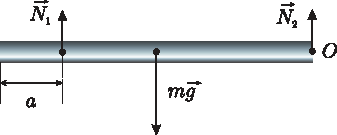
\includegraphics[width=0.6\linewidth]{2007-lahg-02-lah}
\end{center}

Kuna jõudude summa peab tasakaalu asendis olema võrdne nulliga, siis
\[
N_1 + N_2 - mg = 0.
\]
Jõumomentide võrrand punkti $O$ suhtes (võib valida suvalist punkti) on
\[
N_{1}(l-a)=\frac{m g l}{2},
\]
kust saame
\[
N_{1}=\frac{m g l}{2(l-a)}=\frac{80 \cdot \num{9,8} \cdot 5}{2 \cdot(5-1)}=\SI{490}{N}.
\]
Asendades $N_1$ esimesse võrrandisse, saame avaldise $N_2$ jaoks:
\[
N_{2}=\frac{m g(l-2 a)}{2(l-a)}=\frac{80 \cdot \num{9,8} \cdot(5-2 \cdot 1)}{2 \cdot(5-1)}=\SI{294}{N}.
\]
\fi
}